\chapter{Lecture 9: Functions: domain, range, one-to-one, inverse}
In lecture \ref{lec7} we talked about a function as a process that produces one output for each input (and, before that, we first introduced functions in section \ref{sectionfunctions}). We have spoken about random vairables as functions, and about probability measures as functions, and in lecture \ref{lec8} (in examples \ref{example8.11} and \ref{example8.12}) we plotted some graphs of functions whose outputs were discrete values. In lecture \ref{lec7} we also looked at graphs of rational functions, polynomial functions, power functions, exponential functions, logarithms, and others. In section \ref{symblog} we also spoke (informally) about ``undoing'' functions (or ``inverse'' functions).  \\

\subsection{Example} \label{example9.1}
Below are graphs of $f(x) = x^2, \;\; g(x) = \ln(x - 2),$ and $h(x) = 2 - e^{3x}$. Recall that $\ln(x)$ is alternative notation for $\log_\e(x)$.

\begin{center}
\begin{minipage}{0.3\textwidth}
\begin{center}
	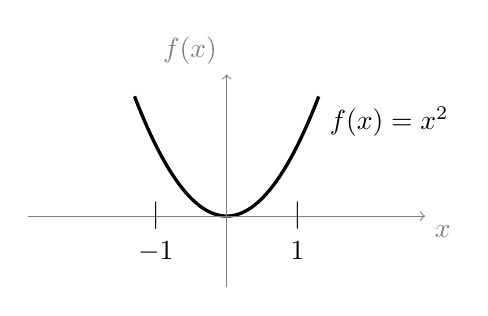
\begin{tikzpicture} [scale = 0.9]
	\draw[very thick, domain = -1.3:1.3, samples=200, smooth] plot (\x,{(\x)^2}) node [below right] {$f(x) = x^2$};
	\draw [gray, ->] (0,-1) -- (0,2) node [above left] {$f(x)$};
	\draw [gray, ->] (-2.8,0) -- (2.8,0) node [below right] {$x$};
	%\draw (3,2) node {Graph of $g(x) = \e^x$};
        %\draw [fill = black] (0,0) circle (0.01cm) node [below left] {$(0,0)$};
	%\node [fill = white] at (pi,1.2) {$f(x) = x^m$};
	%\draw (0,1) [fill = black] circle (0.05cm) node [above right] {$1$};
	\draw (1,0) [fill = black] node {$|$} node [below = 2mm] {$1$};
	\draw (-1,0) [fill = black] node {$|$} node [below = 2mm] {$-1$};
	\end{tikzpicture}
\end{center}
\end{minipage}
\hspace{10mm}
\begin{minipage}{0.3\textwidth}
\begin{center}
	\begin{tikzpicture} [yscale = 0.9,xscale = 0.75]
	\draw[very thick, domain = 1.2:4, samples=200, smooth] plot (\x,{ln(\x-1)}) node [below right] {$g(x) = \ln(x-2)$};
	\draw [gray, ->] (0,-1) -- (0,1.8) node [above left] {$g(x)$};
	\draw [gray, ->] (-0.1,0) -- (4,0) node [below right] {$x$};
	%\draw (3,2) node {Graph of $g(x) = \e^x$};
        %\draw [fill = black] (0,0) circle (0.01cm) node [below left] {$(0,0)$};
	%\node [fill = white] at (pi,1.2) {$f(x) = x^m$};
	\draw (1,0) [fill = black] node {$|$} node [below = 2mm] {$2$};
	\draw (2,0) [fill = black] node {$|$} node [below = 2mm] {$3$};
	\end{tikzpicture}
\end{center}
\end{minipage}%
\hspace{10mm}
\begin{minipage}{0.3\textwidth}
\begin{center}
	\begin{tikzpicture} [yscale = 0.68,xscale = 1]
	\draw[very thick, domain = -2:0.7, samples=200, smooth] plot (\x,{3 - exp((2*\x))}) node [below right] {$h(x) = 2 - \e^{3x}$};
	\draw [gray, ->] (0,-1) -- (0,4) node [above left] {$h(x)$};
	\draw [gray, ->] (-2.8,0) -- (2.8,0) node [below right] {$x$};
	%\draw (3,2) node {Graph of $g(x) = \e^x$};
        %\draw [fill = black] (0,0) circle (0.01cm) node [below left] {$(0,0)$};
	%\node [fill = white] at (pi,1.2) {$f(x) = x^m$};
	%\draw (0,1) [fill = black] circle (0.01cm) node [above right] {$1$};
	\draw (-0.1,3) -- (0.1,3) node [right] {$2$};
	\draw (1,0) [fill = black] node {$|$} node [below = 2mm] {$1$};
	\end{tikzpicture}
\end{center}
\end{minipage}
\end{center}

Things you should notice (or ask yourself) include:
\begin{itemize}
\item Where is the function defined? i.e., what are its possible input~values~(domain)?
\item What are the possible output values?
\item Does the graph increase or decrease? Neither? Both at different locations?
\end{itemize}

\noindent For example, if we want to find the domain of $\ln(x-2)$ then we can compare this expression to $\ln(x)$. We know from section \ref{symblog} that $\ln(x)$ is undefined whenever $x \leq 0$, so this implies that $\ln(x - 2)$ is undefined wherever $x - 2 \leq 0$. Adding $2$ to both sides of this inequality gives $x \leq 2$. So $\ln(x - 2)$ is undefined wherever $x \leq 2$. In other words, the domain of $\ln(x-2)$ is the set of real numbers that are strictly greater than $2$.

\subsection{Interval notation} \label{interval notation}
In section \ref{interval notation 1}, and in the box in section \ref{cdf}, we briefly introduced some \textbf{interval notation}. Interval notation is very convenient; however, it is important to remember that it only applies to real number intervals (not natural numbers or integers, for example). Below we have listed, side by side, 3 ways of expressing the same interval, $\set{x \in \R \mid a \leq x < b}$:
\begin{center}
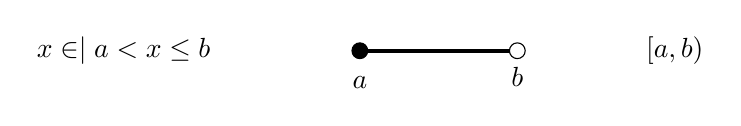
\begin{tikzpicture}
	\draw (0,0) node {$\set{x \in \R \mid a < x \leq b}$};
	\draw [ultra thick] (3,0) -- (5,0);
	\draw [fill = black] (3,0) circle (0.1cm) node [below = 2mm] {$a$};
	\draw [fill = white] (5,0) circle (0.1cm) node [below = 0.8mm] {$b$};
	\draw (7,0) node {$[a,b)$};
\end{tikzpicture}
\end{center}
On the left we have set notation, in the center is a number line representation, and on the right is interval notation, ``$[a,b)$''. The symbol``$\leq$'' in set notation, the black filled circle in the number line representation, and the symbol ``$[$`` (square bracket) in interval notation, all indicate that the interval includes the point $a$. To indicate that $b$ is not included in the interval we use ``$<$'' in set notation, a white filled circle in the diagram notation, and a curly bracket, ``$)$'', in interval notation. Below are more examples of the three notations
\begin{center}
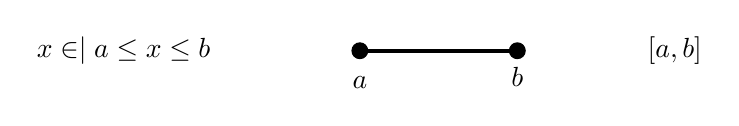
\begin{tikzpicture}
	\draw (0,0) node {$\set{x \in \R \mid a \leq x \leq b}$};
	\draw [ultra thick] (3,0) -- (5,0);
	\draw [fill = black] (3,0) circle (0.1cm) node [below = 2mm] {$a$};
	\draw [fill = black] (5,0) circle (0.1cm) node [below = 0.8mm] {$b$};
	\draw (7,0) node {$[a,b]$};
\end{tikzpicture}
\end{center}
\begin{center}
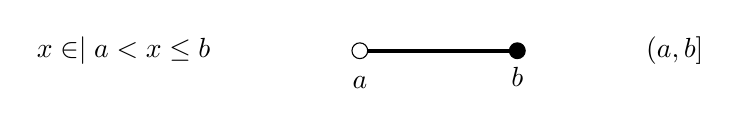
\begin{tikzpicture}
	\draw (0,0) node {$\set{x \in \R \mid a < x \leq b}$};
	\draw [ultra thick] (3,0) -- (5,0);
	\draw [fill = white] (3,0) circle (0.1cm) node [below = 2mm] {$a$};
	\draw [fill = black] (5,0) circle (0.1cm) node [below = 0.8mm] {$b$};
	\draw (7,0) node {$(a,b]$};
\end{tikzpicture}
\end{center}
\begin{center}
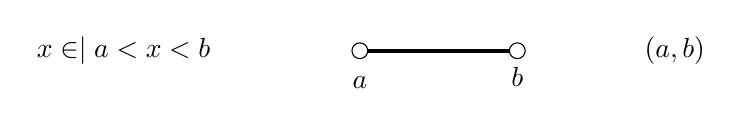
\begin{tikzpicture}
	\draw (0,0) node {$\set{x \in \R \mid a < x < b}$};
	\draw [ultra thick] (3,0) -- (5,0);
	\draw [fill = white] (3,0) circle (0.1cm) node [below = 2mm] {$a$};
	\draw [fill = white] (5,0) circle (0.1cm) node [below = 0.8mm] {$b$};
	\draw (7,0) node {$(a,b)$};
\end{tikzpicture}
\end{center}
If we want to express the set $\set{x \in \R \mid x \leq a}$ in interval notation, we can use the ``$\infty$'' symbol, i.e.,  $\set{x \in \R \mid x \leq a} = (-\infty,a]$. Some more examples:
\[
\set{x \in \R \mid x \geq a} = [a,\infty), \qquad \set{x \in \R \mid x > a} = (a,\infty), \qquad \set{x \in \R \mid x < a} = (-\infty,a).
\]
Suppose that we want to write the interval that has the following number line representation:
\bigskip
\begin{center}
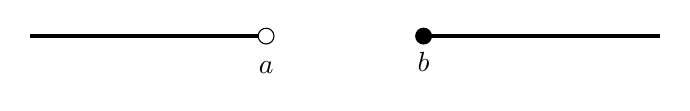
\begin{tikzpicture}
	%\draw (0,0) node {$\set{x \in \R \mid a < x < b}$};
	\draw [ultra thick] (0,0) -- (3,0);
	\draw [ultra thick] (5,0) -- (8,0);
	\draw [fill = white] (3,0) circle (0.1cm) node [below = 2mm] {$a$};
	\draw [fill = black] (5,0) circle (0.1cm) node [below = 0.8mm] {$b$};
	%\draw (7,0) node {$(a,b)$};
\end{tikzpicture}
\end{center}

\noindent This is the set $\set{x \in \R \mid x < a  \text{ or } x \geq b}$. To write it in interval notation, we need to think of this as a union of two sets, i.e., 
\[
\set{x \in \R \mid  x < a  \text{ or } x \geq b} = \set{x \in \R \mid x < a} \cup \set{x \in \R \mid x \geq b}.
\] 
It follows that
\[
\set{x \in \R \mid x \geq b \text{ or } x < a} = (-\infty,a) \cup [b,\infty)
\]
Some other examples of sets of this type are
\begin{center}
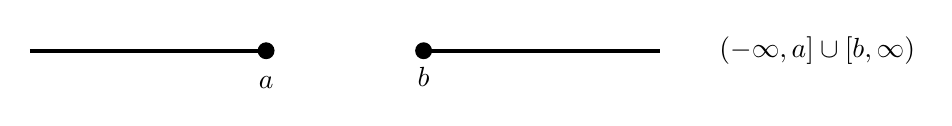
\begin{tikzpicture}
	%\draw (0,0) node {$\set{x \in \R \mid a < x < b}$};
	\draw [ultra thick] (0,0) -- (3,0);
	\draw [ultra thick] (5,0) -- (8,0);
	\draw [fill = black] (3,0) circle (0.1cm) node [below = 2mm] {$a$};
	\draw [fill = black] (5,0) circle (0.1cm) node [below = 0.8mm] {$b$};
	%\draw (7,0) node {$(a,b)$};
	\draw (10,0) node {$(-\infty,a] \cup [b,\infty)$};
\end{tikzpicture}
\end{center}
\begin{center}
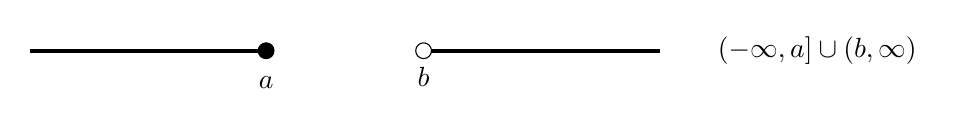
\begin{tikzpicture}
	%\draw (0,0) node {$\set{x \in \R \mid a < x < b}$};
	\draw [ultra thick] (0,0) -- (3,0);
	\draw [ultra thick] (5,0) -- (8,0);
	\draw [fill = black] (3,0) circle (0.1cm) node [below = 2mm] {$a$};
	\draw [fill = white] (5,0) circle (0.1cm) node [below = 0.8mm] {$b$};
	%\draw (7,0) node {$(a,b)$};
	\draw (10,0) node {$(-\infty,a] \cup (b,\infty)$};
\end{tikzpicture}
\end{center}
\begin{center}
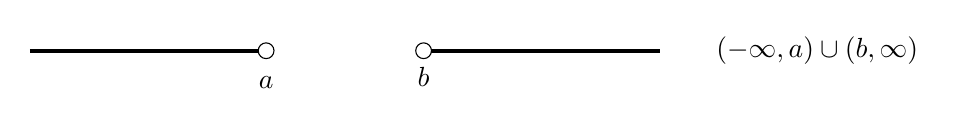
\begin{tikzpicture}
	%\draw (0,0) node {$\set{x \in \R \mid a < x < b}$};
	\draw [ultra thick] (0,0) -- (3,0);
	\draw [ultra thick] (5,0) -- (8,0);
	\draw [fill = white] (3,0) circle (0.1cm) node [below = 2mm] {$a$};
	\draw [fill = white] (5,0) circle (0.1cm) node [below = 0.8mm] {$b$};
	%\draw (7,0) node {$(a,b)$};
	\draw (10,0) node {$(-\infty,a) \cup (b,\infty)$};
\end{tikzpicture}
\end{center}
Notice that, in interval notation, we never \textit{include infinity} in the interval (we never write square brackets next to the infinity symbol); this is because infinity is not a number. It makes no sense to include infinity in an interval (since this would indicate that we are treating infinity as if it were a single point); hence, we always use curly brackets, ``(`` or ``)'', next to the infinity symbol in interval notation. \\

\noindent In general, we can use a variable (usually the letter $I$) to refer to an arbitrary interval; this is useful if it is not important to specify exactly what the interval is, or if we need to state a fact which holds for all intervals of some type.

\subsection{Example}
We define three functions as in example \ref{example9.1}: 
\begin{align*}
f(x) & = x^2; \\
g(x) & = \ln(x - 2); \\
h(x) & = 2 - \e^{3x}.
\end{align*}
Now, try to do the following tasks before looking at the answers:
\begin{itemize}
\item Write down the domain of $g(x)$ using interval notation;
\item Write down the possible outputs of $f(x)$ using interval notation;
\item Write the possible outputs of $h(x)$ using interval notation.
\end{itemize}
\bigskip
\textit{Solutions:}
\begin{align*}
&\text{The domain of $g(x)$ is $(2,\infty)$}; \tag{As explained in example \ref{example9.1}}\\
&\text{The outputs of $f(x)$ are $[0,\infty)$}; \tag{Since squares are always positive} \\
&\text{The outputs of $h(x)$ are $(-\infty,2)$}. \tag{Since $\e^{3x}$ can get arbitrarily close to zero}
\end{align*}

\section{Inverse functions} \label{inverse functions 3}
It was briefly discussed in section \ref{symblog} that if some function, $f$, has an inverse function, then this inverse function ``undoes'' the behaviour of $f$. However, not all functions have inverses, and it will be useful to be able to tell when a function definitely does have an inverse. So, before we define formally what an inverse function is, we will describe exactly which kinds of functions always have inverses. This will also prepare us to better understand the formal definition of inverse functions.

\subsection{codomain vs range}
In section \ref{sectionfunctions} on page \pageref{sectionfunctions} we introduced the terms \textbf{codomain} and \textbf{range}; if you are not already very comfortable with these two terms, then you are encouraged to go back and read that section again now. In a nutshell, the set of all possible output values of a function are called its \textbf{range}.


\subsection{one-to-one functions} \label{one to one}
In section \ref{sectionfunctions} we saw a diagram of a function, $g$, which produced the same output, `red', for more than one input. We had $g(2) = `\text{red}', \; g(5) = `\text{red}'$, and $g(7) = `\text{red}'.$ The arrow diagram of $g$ looked like this:
\begin{center}
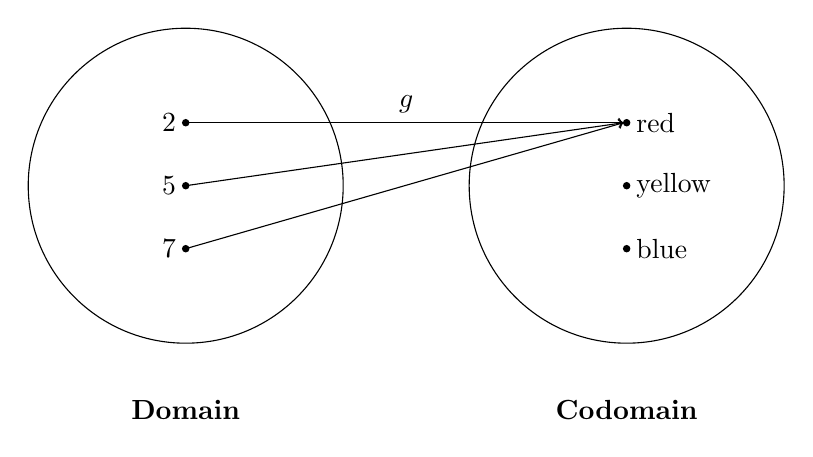
\begin{tikzpicture} [scale = 0.8]
	\draw (0,0) circle (2.5cm) node [below = 2.6cm] {\textbf{Domain}};
	\draw (7,0) circle (2.5cm) node [below = 2.6cm] {\textbf{Codomain}};
	\draw [->] (0,0) -- (7-0.05,1);
	\draw [->] (0,1) -- (7-0.05,1);
	\draw [->] (0,-1) -- (7-0.05,1);
	\draw [fill = black] (0,1) circle (0.05cm) node [left] {$2$};
	\draw [fill = black] (0,0) circle (0.05cm) node [left] {$5$};
	\draw [fill = black] (0,-1) circle (0.05cm) node [left] {$7$};
	\draw [fill = black] (7,1) circle (0.05cm) node [right] {red};
	\draw [fill = black] (7,0) circle (0.05cm) node [right] {yellow};
	\draw [fill = black] (7,-1) circle (0.05cm) node [right] {blue};
	\draw (3.5,1) node [above] {$g$};
\end{tikzpicture}
\end{center}
\noindent Suppose that we pick a particular output value of some function and then we ask which input produced it. In the case of $g$, this question does not make sense; there is no unique input which produces `red.' As we will soon see, this is a useful question to be able to ask; so, we would like to give a name to the types of functions for which this question does make sense. The following function, $f$, is one for which the question does make sense:
\begin{center}
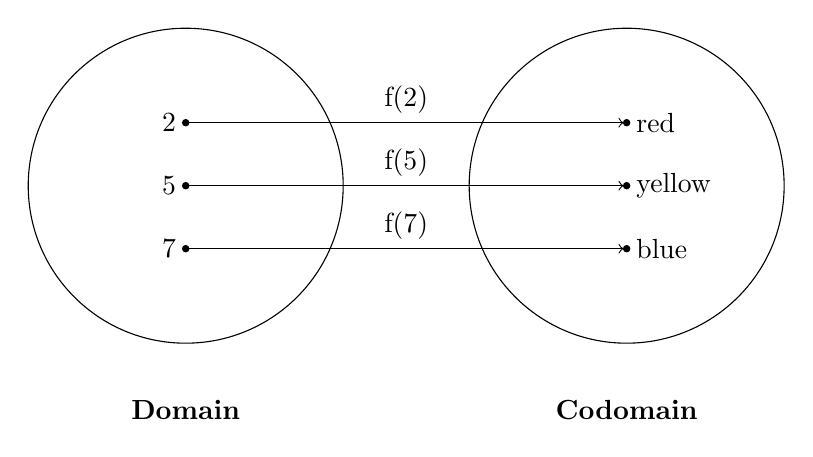
\begin{tikzpicture} [scale = 0.8]
	\draw (0,0) circle (2.5cm) node [below = 2.6cm] {\textbf{Domain}};
	\draw (7,0) circle (2.5cm) node [below = 2.6cm] {\textbf{Codomain}};
	\draw [->] (0,0) -- (7-0.05,0);
	\draw [->] (0,1) -- (7-0.05,1);
	\draw [->] (0,-1) -- (7-0.05,-1);
	\draw [fill = black] (0,1) circle (0.05cm) node [left] {$2$};
	\draw [fill = black] (0,0) circle (0.05cm) node [left] {$5$};
	\draw [fill = black] (0,-1) circle (0.05cm) node [left] {$7$};
	\draw [fill = black] (7,1) circle (0.05cm) node [right] {red};
	\draw [fill = black] (7,0) circle (0.05cm) node [right] {yellow};
	\draw [fill = black] (7,-1) circle (0.05cm) node [right] {blue};
	\draw (3.5,1) node [above] {f(2)};
	\draw (3.5,0) node [above] {f(5)};
	\draw (3.5,-1) node [above] {f(7)};
\end{tikzpicture}
\end{center}
This function is defined so that $f(2) = \set{\text{red}}, \; f(5) = \set{\text{yellow}}$ and $f(7) = \set{\text{blue}}.$ For each possible output there is one unique input. We will call this type of function \textbf{one-to-one}; because it maps one element in the domain to only one element in the range. In the case of $f$ I can ask, ``which input produced `red'?'' Since $f$ is one-to-one, the answer points to just one value in the domain: ``2.''  \\

\noindent If a function, like $g$, is not one-to-one, we can always restrict the domain of that function to ensure that each output matches up with only one input. For example, we could restrict the domain of $g$ from the set $\set{2,5,7}$ to the set $\set{2}.$ Then the arrow diagram of this new function, $g_2$, becomes
\begin{center}
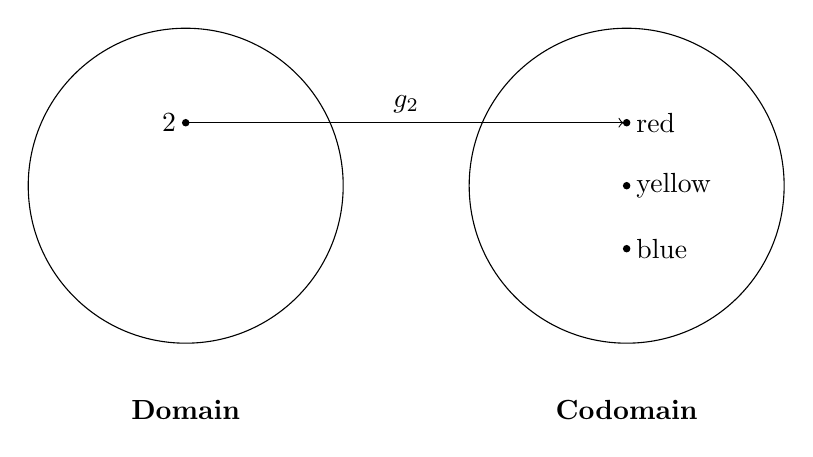
\begin{tikzpicture} [scale = 0.8]
	\draw (0,0) circle (2.5cm) node [below = 2.6cm] {\textbf{Domain}};
	\draw (7,0) circle (2.5cm) node [below = 2.6cm] {\textbf{Codomain}};
	\draw [->] (0,1) -- (7-0.05,1);
	\draw [fill = black] (0,1) circle (0.05cm) node [left] {$2$};
	\draw [fill = black] (7,1) circle (0.05cm) node [right] {red};
	\draw [fill = black] (7,0) circle (0.05cm) node [right] {yellow};
	\draw [fill = black] (7,-1) circle (0.05cm) node [right] {blue};
	\draw (3.5,1) node [above] {$g_2$};
\end{tikzpicture}
\end{center}
As we can see from the diagram, $g_2$ is one-to-one. \\

\noindent Formally, a function $h$ with domain $X$ is one-to-one if whenever we pick two separate (i.e., non-equal) elements from the domain, they never map to the same thing in the range. So, in other words, if we pick $x,y \in X$ (where $x$ and $y$ are not the same element) then we must always have $f(x) \neq f(y)$. Stated again, the \textbf{definition of one-to-one is}: For all $x,y \in X$,

\bigskip

\hfil\fbox{
\begin{minipage}{0.4\columnwidth}{

\vskip 0.02cm
\begin{center}
$x \neq y$ \;\;\; \text{implies} \;\;\; $f(x) \neq f(y)$.
\end{center}
}
\end{minipage}}
\bigskip



\noindent Functions whose domain is a subset of the real numbers, and which are always increasing (or decreasing), for all values in their domain, will always be one-to-one. To understand this, look at the definition of an increasing function; a function, $k$, with domain $X$, where $X$ is a subset of $\R$, is increasing if for all $a,b \in X$,
\[
a > b \;\;\; \text{implies} \;\;\; k(a) > k(b).  
\]
Now, if we pick any pair $x,y$ (with $x \neq y$) from the domain of an increasing function, $k$, then we must have $x > y$ or $y > x$. So, since $k$ is increasing it follows that $k(x) > k(y)$ or $k(y) > k(x)$. In both cases $k(x) \neq k(y)$ (since `$>$' excludes the possibility of `$=$'). So, we have shown that $x \neq y$ implies $k(x) \neq k(y)$. Hence we have shown that the definition of one-to-one is satisfied by $k$; so $k$ is one-to-one.

\subsection{Example}
Name some possible domains on which $f(x) = x^2$ is one-to-one. State the corresponding range. Try to do this before looking at the solution. \\

\noindent \textit{Solution:} \\
\noindent One domain on which $f(x)$ is one-to-one is the interval $[0,\infty)$, i.e. the non-negative real numbers; this is because there are no two (different) non-negative real numbers which, when squared, give you the same result. The corresponding range is $[0,\infty)$. \\

\noindent Another domain on which $f(x)$ is one-to-one is the interval $(-\infty,0]$, i.e., the non-positive real numbers; this is because there are no to two (different) non-positive real numbers which, when squared, give you the same result. The corresponding range is again $[0,\infty)$ (because squaring negative numbers gives positive numbers). \\

\noindent The function $f$ is not one-to-one on the domain $\R$. This is because we can find a pair of (different) elements, for example $-1$ and $1$, which when squared give the same result. That is, $f(-1) = 1$ and $f(1) = 1$ so $f(-1) = f(1)$; so the definition of one-to-one is not satisfied by $f$ if we choose $\R$ as the domain.

\subsection{Composition of functions} \label{composition (of functions)}
Before we get into the definition of inverse functions, we will need to (briefly) learn about composition of functions. Composing functions is a matter of plugging the output of one function into the input of another function. Put simply, if we have two functions, $f(x)$ and $g(x)$, then we can easily evaluate $g(x)$ first, and plug this number into the input of $f(x)$. To indicate that this is what we want to do, we write

\bigskip

\hfil\fbox{
\begin{minipage}{0.15\columnwidth}{

\vskip 0.02cm
\begin{center}
$f(g(x))$
\end{center}
}
\end{minipage}}
\bigskip

\noindent We read this as, ``$f$ of $g$ of $x$.'' For example, suppose $g(x) = x^2$ and $f(x) = x-1$. If we want to find $f(g(2))$ then we start by finding $g(2) = 2^2 = 4$; we then plug this result into $f(x)$ to get $f(4) = 4 - 1 = 3$. Hence $f(g(2)) = 3$. We can find a rule for $f(g(x))$ by plugging the rule for $g(x)$ into the rule for $f(x)$. We get
\begin{align*}
f(g(x)) & = g(x) - 1 \tag{since $f(x) = x-1$} \\
	 & = x^2 - 1 \tag{since $g(x) = x^2$}
\end{align*}
Now we can check that $f(g(2)) = 2^2 - 1 = 4 - 1 = 3$, as required.

\subsection{Definition of inverse function}
Say that we have some function, $f$, which is one-to-one, and has the following graph:
\begin{center}
\begin{tikzpicture}[yscale = 2.5,xscale=2.7]
	\draw[very thick, domain = -0.1:1.8, samples=200, smooth] plot (\x,{-exp(-(\x)^3) + 1});
	\draw [gray, ->] (0,-0.2) -- (0,1.5) node [above left] {$f(x)$};
	\draw [gray, ->] (-0.2,0) -- (2.4,0) node [below right] {$x$};
\end{tikzpicture}
\end{center}
\noindent Suppose we want to take a value, $y_1$, from the range of a one-to-one function function, $f$, and find the input value, $x_1$, which produced it. We can draw this idea quite easily using the graph:
\begin{center}
\begin{tikzpicture}[yscale = 2.5,xscale=2.7]
	\draw[very thick, domain = -0.1:1.8, samples=200, smooth] plot (\x,{-exp(-(\x)^3) + 1});
	\draw [gray, ->] (0,-0.2) -- (0,1.5) node [above left] {$f(x)$};
	\draw [gray, ->] (-0.2,0) -- (2.4,0) node [below right] {$x$};
	\draw (0.9,0) [fill = black] node {$|$} node [below = 2mm] {$x_1$};
	\draw [thick, dashed] (0,0.5) -- (0.9,0.5);
	\draw [thick, dashed, ->] (0.9,0.5) -- (0.9,0);
	\draw (0.05,0.5) -- (-0.05,0.5) node [left] {$y_1$};
\end{tikzpicture}
\end{center}
We can see from the graph that $f(x_1) = y_1$; so, $x_1$ is the input which produced $y_1$. This process of asking which input produced each output is itself a function. We will label it $f^{-1}$, which is read as ``$f$ inverse.'' So if we write, ``what is $f^{-1}(y_1)$?'' Then this is equivalent to asking the question, ``which input in the domain of $f$ produced $y_1$?'' In this case we have learned from the graph that $f^{-1}(y_1) = x_1$. \\

\noindent \textbf{The domain of $\boldsymbol{f^{-1}}$ is the range of the original function, $\boldsymbol{f}$, and the range of $\boldsymbol{f^{-1}}$ is the domain of $\boldsymbol{f}$}. In other words, we can obtain a graph of $f^{-1}$ by first taking the graph of $f$, then interchanging the $x$ and $y$ axes; as a result the graph gets ``mirrored'' in the line $y = x$ as follows:  \\
Start with the graph of $f$:
\begin{center}
\begin{tikzpicture}[scale = 1.5]
	\draw[very thick, domain = -0.1:1.8, samples=200, smooth] plot (\x,{-exp(-(\x)^3) + 1});
	\draw [gray, ->] (0,-0.2) -- (0,2.2) node [above left] {$f(x) = y$};
	\draw [gray, ->] (-0.2,0) -- (2.2,0) node [below right] {$x = f^{-1}(y)$};
	\draw [dashed] (0,0) -- (2.5,2.5) node [above right] {$y = x$};
\end{tikzpicture}
\end{center}
Then interchange the $x$ and $y$ axes,
\begin{center}
\begin{tikzpicture}[scale = 1.5]
\begin{scope}[yscale=-1, xscale = 1, rotate = -90]
	\draw[very thick, domain = -0.1:1.8, samples=200, smooth] plot (\x,{-exp(-(\x)^3) + 1});
	\draw [gray, ->] (0,-0.2) -- (0,2.2) node [below right] {$y$};
	\draw [gray, ->] (-0.2,0) -- (2.2,0) node [above left] {$f^{-1}(y)$};
	\draw [dashed] (0,0) -- (2.5,2.5) node [above right] {$y = x$};
\end{scope}
\end{tikzpicture}
\end{center}
You should be able to tell that the new graph is like a reflection of the old graph accross the dashed line $y = x$. \\

\noindent Now that we can take the inverse of any one-to-one function, $f$, we can also take the inverse of the \textit{inverse} function $f^{-1}$. In other words we can ask, what is $\brac{f^{-1}}^{-1}\brac{x_1}$? This is equivalent to asking, ``what is the number in the domain of $f^{-1}$ which gives the output $x_1$?'' Earlier we found out (from the graph of $f$) that $f^{-1}(y_1) = x_1$. So, the input which produced $x_1$ was $y_1$. This means that $\brac{f^{-1}}^{-1}(x_1) = y_1$. On the graph of $f$ this looks as follows:
\begin{center}
\begin{tikzpicture}[yscale = 2.5,xscale=2.7]
	\draw[very thick, domain = -0.1:1.8, samples=200, smooth] plot (\x,{-exp(-(\x)^3) + 1});
	\draw [gray, ->] (0,-0.2) -- (0,1.5) node [above left] {$f(x)$};
	\draw [gray, ->] (-0.2,0) -- (2.4,0) node [below right] {$x$};
	\draw (0.9,0) [fill = black] node {$|$} node [below = 2mm] {$x_1$};
	\draw [thick, dashed, <-] (0,0.5) -- (0.9,0.5);
	\draw [thick, dashed] (0.9,0.5) -- (0.9,0);
	\draw (0.05,0.5) -- (-0.05,0.5) node [left] {$y_1$};
\end{tikzpicture}
\end{center}
But we can see from the graph that this process gives the same result as $f(x)$. So, we can conclude that $\brac{f^{-1}}^{-1}(x) = f(x)$. In other words the inverse function of $f^{-1}$ is just the original function, $f$. This is, of course, to be expected. We can now refer to the functions $f$ and $f^{-1}$ as inverse to \textit{eachother}. The following two conditions, (i) and (ii), are another way of stating what we have just learned about inverse functions. (i) and (ii) can be taken together as the \textbf{definition of inverse functions:} \\
\bigskip

\hfil\fbox{
\begin{minipage}{0.7\columnwidth}{

\vskip 0.02cm
\begin{center}
$(\text{i}) \;\;\; f^{-1}\brac{f(x)} = x$ \;\;\;\;\;\; and \;\;\;\;\;\; $(\text{ii}) \;\;\; f\brac{f^{-1}(y)} = y$.
\end{center}
}
\end{minipage}}
\bigskip

\noindent We can use (i) to help us find a rule for the inverse of a given function (see the example below).

\subsection{Example} \label{ex9.inverse}
Find the inverse function of $g(x) = \ln(x-2)$ from example \ref{example9.1}. \\

\noindent \textit{Solution:} \\
\noindent The trick is to let $g(x) = y$, then use (i) from the above definition of inverse functions, as follows: \\
\bigskip
\noindent Let $g(x) = y$. Then
\[
g^{-1}(y) = g^{-1}(g(x)) = x. \tag{by (i)}
\]
So now we know that $g^{-1}(y) = x$, which is the key fact that we use to find the inverse during the following steps: \\
We have,
\begin{alignat*}{2}
&& g(x) 
& = y \\
& \iff 
& \ln(x-2)  
& = y \tag{since $g(x) = \ln(x-2)$} \\
& \iff 
& e^{\ln(x - 2)} & = e^y \\
& \iff 
& (x-2) 
& = e^y \tag{using logarithm property (i) from section \ref{symbln}} \\
& \iff
& x
& = e^y + 2 \tag{adding $2$ to both sides}
\end{alignat*}
Here is where we use the fact that $g^{-1}(y) = x$. Replacing $x$ with $g^{-1}(y)$ in $x = e^y + 2$ gives,
\[
g^{-1}(y) = e^y + 2.
\]
We are now done, as we have found an expression for $g^{-1}$.
Since $y$ is a just a ``dummy variable'' we can replace it with whichever variable we like, so we can rewrite $g^{-1}$ as
\[
g^{-1}(x) = e^x + 2, \;\;\; \text{where $x \in \R$.}
\]
\bigskip
\textit{Note:} \\
According to condition (i) from the defintion of inverse functions, we should find that $g^{-1}(g(x)) = x$. We can check that this is true given our expression for $g^{-1}$. We have,
\begin{align*}
g^{-1}(g(x)) & = e^{g(x)} + 2 \\
		     & = e^{\ln(x-2)} + 2 \tag{since $g(x) = \ln(x-2)$} \\
		     & = (x - 2) + 2 \tag{using logarithm property (i) from section \ref{symbln}} \\
		     & = x.
\end{align*}
So this gives us confidence that our expression for $g^{-1}$ is correct (a great way to check assignment questions).

\subsection{Definition of square root} \label{square root}
Suppose that we want to solve for $y$ in the equation
\[
x = y^2.
\] 
The solution depends on the domain of $y$. For example, if we have,
\[
4 = y^2.
\]
Then we might have $y = 2$ or $y = -2$. Let $f$ be the squaring function, so that $f(x) = x^2$. Then the following is an arrow diagram of $f$:
\begin{center}
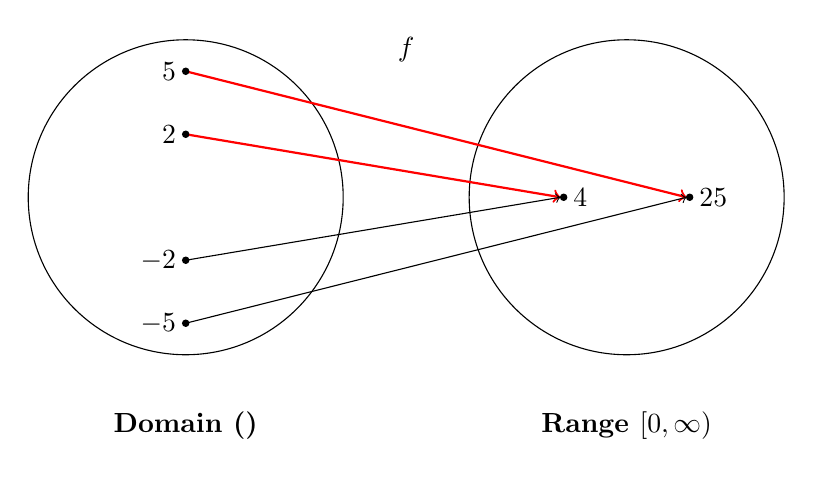
\begin{tikzpicture} [scale = 0.8]
	\draw (0,0) circle (2.5cm) node [below = 2.6cm] {\textbf{Domain ($\R$)}};
	\draw (7,0) circle (2.5cm) node [below = 2.6cm] {\textbf{Range $[0,\infty)$}};
	\draw [thick, red, ->] (0,1) -- (6-0.05,0);
	\draw [thick, red, ->] (0,2) -- (8-0.05,0);
	\draw [->] (0,-1) -- (6-0.05,0);
	\draw [->] (0,-2) -- (8-0.05,0);
	\draw [fill = black] (0,1) circle (0.05cm) node [left] {$2$};
	\draw [fill = black] (0,2) circle (0.05cm) node [left] {$5$};
	\draw [fill = black] (0,-1) circle (0.05cm) node [left] {$-2$};
	\draw [fill = black] (0,-2) circle (0.05cm) node [left] {$-5$};
	\draw [fill = black] (6,0) circle (0.05cm) node [right] {$4$};
	\draw [fill = black] (8,0) circle (0.05cm) node [right] {$25$};
	\draw (3.5,2) node [above] {$f$};
\end{tikzpicture}
\end{center}
Each element in the range of $f$ has two elements, one positive and one negative, mapped to it from the domain. This means that the squaring function is not one-to-one, so it does not have an inverse when $x \in \R$. However, it would be useful to have a kind of pseudo-inverse function for $f$ which asks ``what is the positive number which when squared gives $x$?'' The function which answers this question is called the square root function; if $x = y^2$, then we define $\sqrt{x}$ to mean
\[
\scases{\sqrt{x}}{y}{\text{if} \;\; y \geq 0}{-y}{\text{if} \;\; y < 0}.
\]
This is equivalent to the inverse function of $f$ when $f$ is restricted to the domain $[0,\infty).$ However, using this function we do not need to restrict the domain of $f$. \\

\noindent Now we can find, for example, $\sqrt{(-1)^2}$: We have,
\[
\scases{\sqrt{(-1)^2}}{(-1)}{\text{if} \;\; -1 \geq 0}{-(-1)}{\text{if} \;\; -1 < 0}.
\]
Since $-1$ is less than $0$, we choose the bottom case,
\[
\sqrt{(-1)^2} = -(-1) = 1.
\]
During the solutions to questions (2) and (3) in the following example we use the square root function. As you will see, it is our responsibility to remember that the square root function always returns a positive result. 

\subsection{Example}
Try to do the following tasks before looking at the solutions:
\begin{enumerate}
\item Find $h^{-1}$ for the function $h(x) = 2 - \e^{3x}$ from example \ref{example9.1}.
\item Find the inverse of the function $j(x) = -x^2$
\item Find the inverse of the function $k(x) = (x - 2)^2$ defined on $(-\infty,2].$
\item Find the inverse of the function $\ell(x) = \e^{(x-1)^3} - 5$.
\end{enumerate}
In some steps we will have to take the square root of a variable. While doing this, we need to be careful to remember that the square root function only returns a positive result (see section \ref{square root}). So, for example, if we are solving $y = x^2$, then we need to write $x = \sqrt{y}$ if the domain of $x$ is $[0,\infty),$ otherwise we need to write $x = -\sqrt{y}$ if the domain of $x$ is $(-\infty,0]$. In practice, we can initially write $x = \pm\sqrt{y}$, then later decide whether to choose $+$ or $-$ based on the domain of $x$. \\


\bigskip
\noindent \textbf{\textit{Solution to (1):}} \\ 
Let $x \in \R$. Let $h(x) = y$. Then $y \in (-\infty,2)$ ($y$ must belong to $(-\infty,2)$ since this is the range of $h(x)$). Now,
\[
h^{-1}(y) = h^{-1}\brac{h(x)} = x \tag{by (i) from definition of inverse functions}
\]
Hence $h^{-1}(y) = x$. Now,
\begin{alignat*}{2}
&& h(x) 
& = 2 - \e^{3x} \\
&\iff 
& y 
& = 2 - \e^{3x} \\
&\iff
& \e^{3x}
& = 2 - y \\
& \iff
& \ln(\e^{3x})
& = \ln(2-y) \tag{which is defined, since $y < 2$, so $2-y > 0$} \\
& \iff
& 3x
& = \ln(2-y) \tag{using logarithm property (ii) from section \ref{symbln}}\\
&\iff
& x
& = \frac{1}{3}\ln(2-y). \\
& \iff
& h^{-1}(y)
& = \frac{1}{3}\ln(2-y).
\end{alignat*}
So replacing the dummy variable, $y$, with $x$ we have
\[
h^{-1}(x) = \frac{1}{3}\ln(2-x), \;\;\; \text{where $x \in (-\infty,2)$}
\]
\noindent \textit{Check solution to 1:} \\
\begin{align*}
h^{-1}\brac{h(x)} & = \frac{1}{3}\ln(2-h(x)) \\ 
			      & = \frac{1}{3}\ln\brac{2 - \brac{2-\e^{3x}}} \\
			      & = \frac{1}{3}\ln\brac{\e^{3x}} \\
			      & = \frac{1}{3}\brac{3x} \\
			      & = x.
\end{align*}
This gives us confidence that we didn't make any mistakes. \\

\bigskip
\noindent \textbf{\textit{Solution to (2):}} \\
Let $x \in [0,\infty)$. Let $j(x) = y$. Then $y \in (-\infty,0]$ ($y$ must belong to $(-\infty,0]$ since this is the range of $j(x)$). Now,
\[
j^{-1}(y) = j^{-1}\brac{j(x)} = x \tag{by (i) from definition of inverse functions}
\]
Hence $j^{-1}(y) = x$. Now,
\begin{alignat*}{2}
&& j(x) 
& = -x^2 \\
& \iff 
& y 
& = -x^2 \\
& \iff
& -y 
& = x^2 \\
& \iff
& \pm\sqrt{-y}
& = \sqrt{x^2} \tag{$\sqrt{-y}$ is defined, because $y < 0$ so $-y > 0$} \\
& \iff
& \pm\sqrt{-y}
& = x \tag{since $\sqrt{x^2} = \brac{x^2}^\frac{1}{2} = x^\frac{2}{2} = x$ (index laws)} \\
& \iff
& \sqrt{-y}
& = x \tag{since $x \in [0,\infty)$} \\
& \iff 
& \sqrt{-y}
& = j^{-1}(y) \tag{since $x = j^{-1}(y)$}.
\end{alignat*}
Notice that we chose the positive square root because $x \in [0,\infty)$. Replacing the dummy variable, $y$, with $x$ gives
\[
j^{-1}(x) = \sqrt{-x}, \;\;\; \text{where $x \in (-\infty,0]$}
\]
\noindent\textit{Check solution 2:} \\
We have,
\begin{align*}
j^{-1}\brac{j(x)} & = \sqrt{-j(x)} \\
			    & = \sqrt{-\brac{-x^2}} \\
			    & = \sqrt{x^2} \\
			    & = x.
\end{align*}
This gives us confidence that we didn't make any mistakes. \\

\bigskip
\noindent \textbf{\textit{Solution to (3):}} \\
Let $x \in (-\infty,2]$. Let $k(x) = y$. Then $y \in [0,\infty)$ (y must belong to $[0,\infty)$ since this is the range of $k(x)$). Now,
\[
k^{-1}(y) = k^{-1}\brac{k(x)} = x \tag{by (i) from definition of inverse functions}
\]
Hence $k^{-1}(y) = x$. Now,
\begin{alignat*}{2}
&& k(x)
&  = (x-2)^2 \\
& \iff
& y
& = (x-2)^2  \\
& \iff
& \pm\sqrt{y}
& = \sqrt{\brac{x - 2}^2} \tag{$\sqrt{y}$ is defined since $y\geq0$} \\
& \iff
& \pm\sqrt{y}
& = x - 2 \tag{since $\sqrt{\brac{x - 2}^2} = \brac{x - 2}^\frac{2}{2} = x - 2$ (index laws)} \\
& \iff
& - \sqrt{y}
& = x - 2 \tag{since $x \in (-\infty,2]$ so $x-2 \in (-\infty,0]$} \\
& \iff
& 2-\sqrt{y}
& = x \\
& \iff 
& 2 - \sqrt{y} 
& = k^{-1}(y) \tag{since $x = k^{-1}(y)$}
\end{alignat*}
Notice that we chose the negative square root because $x - 2 \in (-\infty,0]$. Replacing the dummy variable, $y$, with $x$ we have
\[
k^{-1}(x) = 2 - \sqrt{x}.
\]
\noindent\textit{Check solution to 3:} \\
We have
\begin{align*}
k^{-1}\brac{k(x)} & = 2 - \sqrt{k(x)} \\
			     & = 2 - \sqrt{(x-2)^2} \\
			     & = 2 - (2-x) \tag{$\star$} \\
			     & = x.
\end{align*}
The step labelled ($\star$) might have seemed confusing, but this confusion can be alleviated by looking at the definition of square root from section \ref{square root}:
\[
\scases{\sqrt{x^2}}{x}{x \geq 0}{-x}{x < 0}
\]
So if we look at $\sqrt{\brac{x-2}^2}$ using this definition we have,
\[
\scases{\sqrt{\brac{x-2}^2}}{(x-2)}{x-2\geq0}{-(x-2)}{x-2 < 0}
\]
Since $x \leq 2$ we know that $x-2 \leq 0$. So, we conclude that $\sqrt{\brac{x-2}^2} = -(x-2) = 2-x$, which is what we had in $(\star)$. \\

\bigskip
\noindent \textbf{\textit{Solution to (4):}} \\
Let $x \in \R$. Let $\ell(x) = y$. Then $y \in (-5,\infty)$ ($y$ must belong to $(-5,\infty)$ since this is the range of $\ell(x)$). Now,
\[
\ell^{-1}(y) = \ell^{-1}\brac{\ell(x)} = x \tag{by (i) from definition of inverse functions}
\]
Hence $\ell^{-1}(y) = x$. Now,
\begin{alignat*}{2}
&& \ell(x) 
& = \e^{(x-1)^3} - 5 \\
& \iff
& y
& = \e^{(x-1)^3} - 5 \\
& \iff
& y + 5
& = \e^{(x-1)^3} \\
& \iff
& \ln(y + 5)
& = \ln\brac{\e^{(x-1)^3}} \tag{$\ln(y + 5)$ is defined, since $y \in (-5,\infty)$} \\
& \iff
& \ln(y + 5)
& = (x-1)^3 \tag{using logarithm property (ii) from section \ref{symbln}} \\
& \iff
& \brac{\ln(y+5)}^\frac{1}{3}
& = \brac{(x-1)^3}^\frac{1}{3} \\
& \iff
& \brac{\ln(y+5)}^\frac{1}{3}
& = (x-1)  \tag{since $\brac{(x-1)^3}^\frac{1}{3} = (x-1)^\frac{3}{3} = x - 1$ (index laws)} \\
& \iff
& \brac{\ln(y+5)}^\frac{1}{3} + 1 
& = x \\
& \iff
& \brac{\ln(y+5)}^\frac{1}{3} + 1
& = k^{-1}(y). \tag{since $x = k^{-1}(y)$}
\end{alignat*}
Now, replacing the dummy variable, $y$, with $x$ we get
\[
 k^{-1}(x) = \brac{\ln(x+5)}^\frac{1}{3} + 1, \;\;\; \text{where $x \in (-5,\infty).$}
\]
You are encouraged to do the check step to reinforce that this is the correct expression.

%APPLICATIONS: THE INVERSE CAN BE USED TO FIND QUANTILES OF A CDF AS LONG AS THE CDF IS STRICTLY INCREASING. IT IS USED TO GENERATE RANDOM VARIABLES WITH A CDF.